\subsection{Spherical space}
Playing the video game in spherical space gives the impression that the terrain is wallpapered onto the inside of a giant sphere.
Unlike the hyperbolic space, the spherical space is finite.
Comparison in \autoref{fig:spherical-space-games} shows that our implementation provides visual effects to a certain degree similar to those in \textit{Hyperbolica}.
\begin{figure*}[h]
    \centering
    \begin{subfigure}[b]{0.475\textwidth}
        \centering
        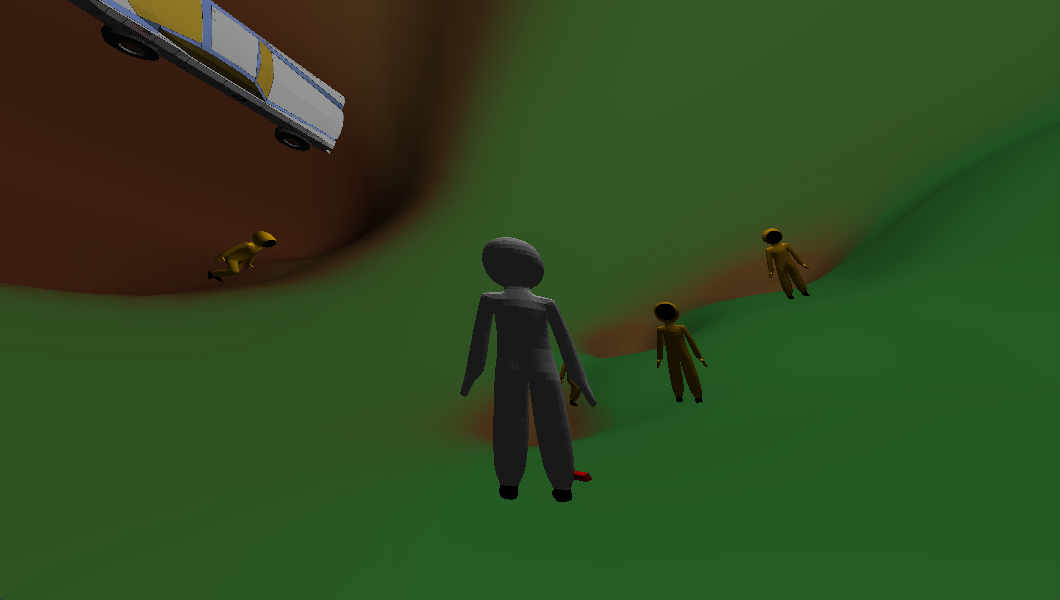
\includegraphics[width=\textwidth]{chapters/results/sections/non_euclidean/resources/spherical-in-hyper.png}
        \caption[]%
        {{\small \textit{Hyper}}}
        \label{fig:spherical-space-games-hyper}
    \end{subfigure}
    \hfill
    \begin{subfigure}[b]{0.5\textwidth}
        \centering
        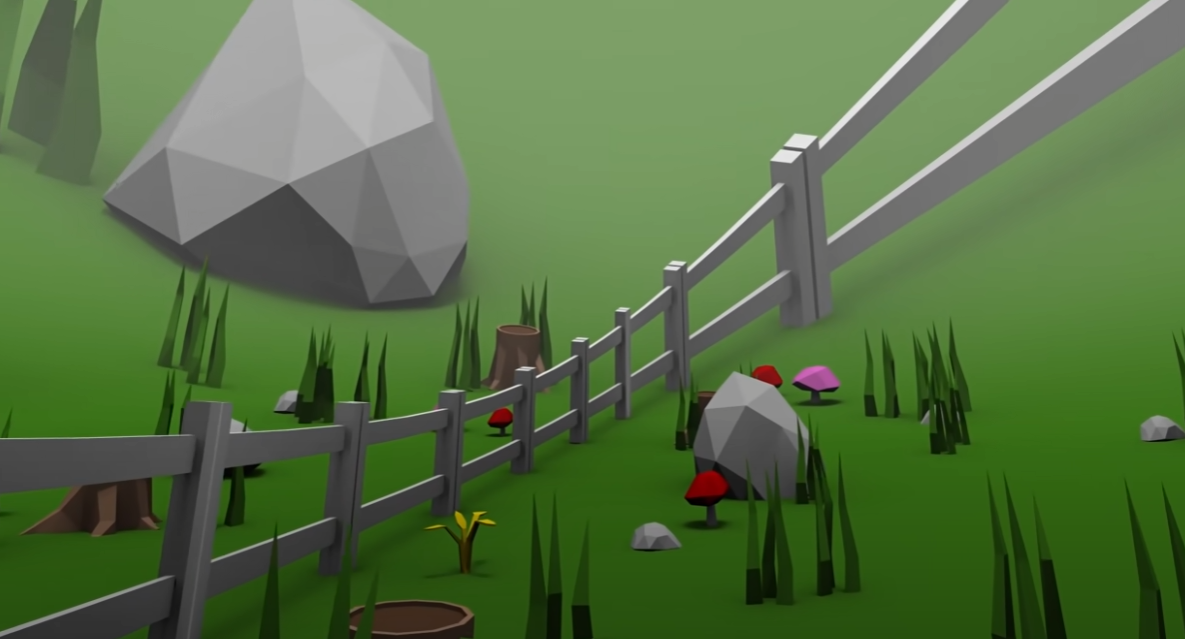
\includegraphics[width=\textwidth]{chapters/results/sections/non_euclidean/resources/hyperbolica-1.png}
        \caption[]%
        {{\small \textit{Hyperbolica \cite{Hyperbolica-Spherical}}}}
        \label{fig:spherical-space-games-hyperbolica}
    \end{subfigure}
    \caption[]
    {\small Spherical space}
    \label{fig:spherical-space-games}
\end{figure*}